\documentclass[slidestop,compress,mathserif,10pt]{beamer}

\mode<article> % 仅应用于article版本
{
  \usepackage{beamerbasearticle}
%  \usepackage{fullpage}
  \usepackage{hyperref}
}

%% 下面的包控制beamer的风格,可以根据自己的爱好修改
\usepackage{beamerthemesplit}   % 使用split风格
\usepackage{beamerthemeshadow}  % 使用shadow风格
%\usepackage[width=2cm,dark,tab]{beamerthemesidebar}
%\usepackage{beamerthemetree}
%\usetheme{Montpellier}
%\usecolortheme{lily}


%% 这些包是可能会用到的,不必修改
\usepackage{amsmath,amssymb}
\usepackage{graphicx}
%\usepackage{color}
%\usepackage{pgf,pgfarrows,pgfnodes,pgfautomata,pgfheaps}
%\usepackage{multimedia}

%\documentclass{beamer}
%\usepackage{beamerthemeshadow}
\usepackage{beamerthemesplit}
%\usetheme{shadow}
\usepackage{graphicx}
\usecolortheme{lily}
%\usepackage{amsmass}
\usepackage{amssymb,amsfonts,url}
\graphicspath{{Problems/}}

%\usepackage{CJK}
%\usepackage{pinyin}

%    \begin{figure}
%        \centering
%        \includegraphics[width=0.8\textwidth]{newGeneRep.eps}
%    \end{figure}

% \begin{figure}%
%   \begin{center}%
%     \begin{minipage}{0.70\textwidth}%
%      \includegraphics[width=1.0\textwidth]{comp25000.eps}%
%     \end{minipage}%
%     \begin{minipage}{0.30\textwidth}
%      \includegraphics[width=1.0\textwidth]{comparelabel.eps}%
%     \end{minipage}%
%   \end{center}
% \end{figure}

% \begin{table}
%   {\begin{tabular}{l|rrr}\hline
%       & \multicolumn{3}{c}{Actual number of DCJ operations}\\
%       \# genes &\# genes $\times 1$&\# genes $\times 2$&\# genes  $\times 3$ \\
% \hline
%      (a)~25,000 & 0.5\% ~~&  0.9\% ~~& 1.7\%~~\\
%       (b)~10,000 & 0.8\%~~ &  1.4\% ~~& 2.7\%~~\\
%      (c)~ 1,000 & 2.7\%~~ & 4.7\%~~ & 14.7\%~~\\ \hline
%     \end{tabular}} {}%
% \end{table}

% \begin{eqnarray}
% T(n) &=&  \sum\nolimits_{i=1}^n C_i \\
%      &=&  \# PUSH + \#POP \\
%      &<& 2\times \#PUSH \\
%      &<& 2n \\
% \end{eqnarray}

% \[ 
% \begin{matrix}
% \begin{pmatrix}
% C_{11} & C_{12} \\ 
% C_{21} & C_{22} 
% \end{pmatrix}
% =
% \begin{pmatrix}
% A_{11} & A_{12} \\ 
% A_{21} & A_{22}  
% \end{pmatrix}
% 
% \begin{pmatrix}
% B_{11} & B_{12} \\ 
% B_{21} & B_{22}  
%  
% \end{pmatrix}
%     
%    \end{matrix}
% \]
% 
% 
% \begin{eqnarray}
%  C_{11} &=& (A_{11}\times B_{11}) + (A_{12} \times B_{21}) \\
% C_{12} &=& (A_{11}\times B_{12}) + (A_{12} \times B_{22}) \\
% C_{21} &=& (A_{21}\times B_{11}) + (A_{22} \times B_{21}) \\
% C_{22} &=& (A_{21}\times B_{12}) + (A_{22} \times B_{22}) 
% \end{eqnarray}
% \begin{figure}%
%      \begin{minipage}{0.32\textwidth}%
%       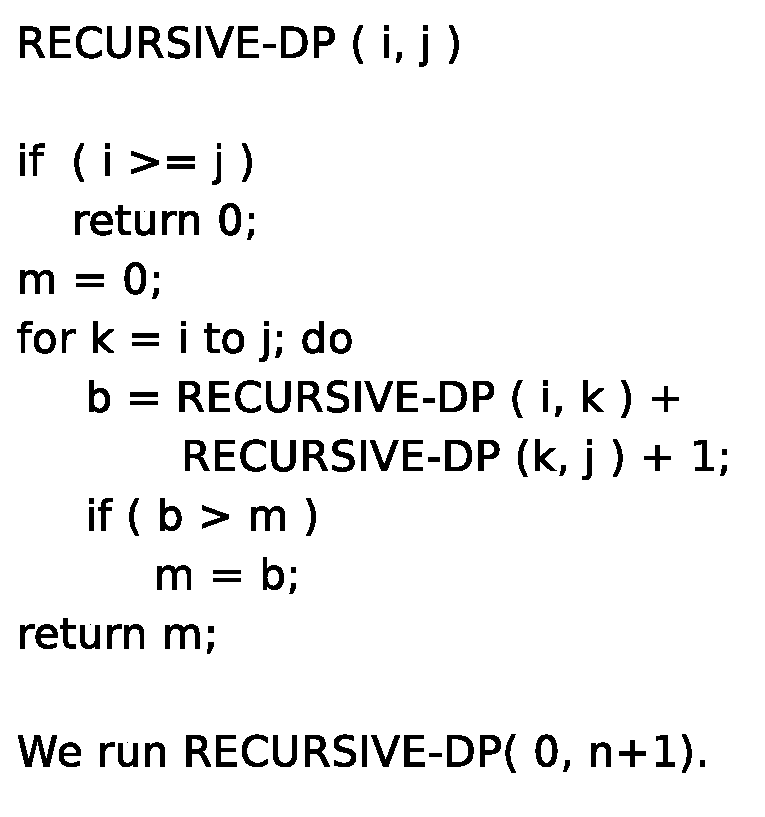
\includegraphics[width=1.0\textwidth]{L7-intervalschedulingdpalgo.eps}%
%      \end{minipage}%
%  \quad
%      \begin{minipage}{0.30\textwidth}
%       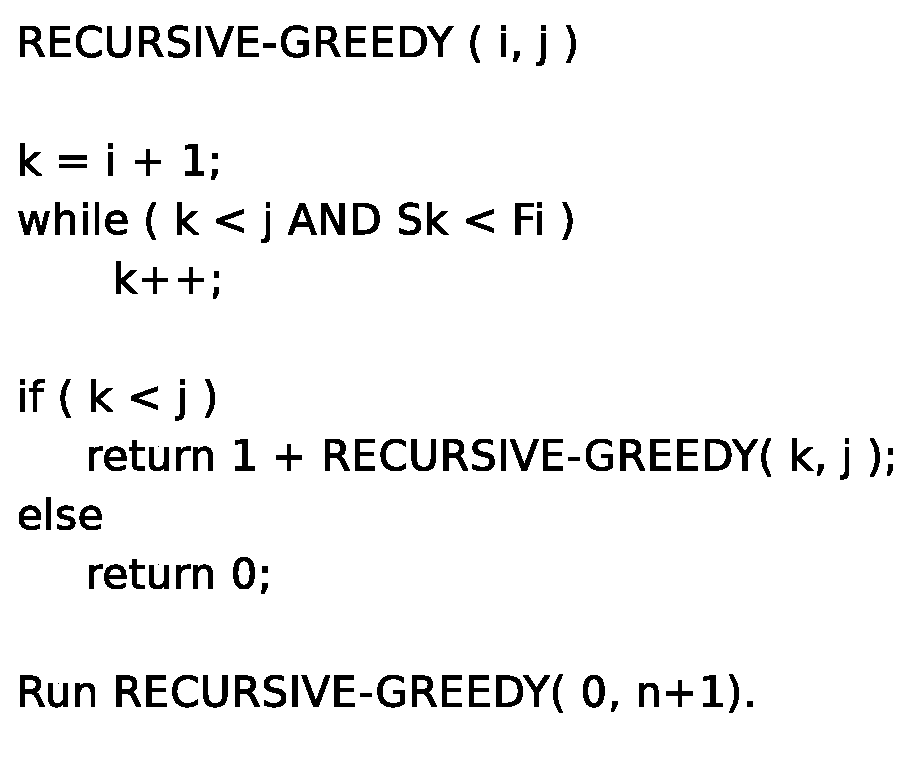
\includegraphics[width=1.0\textwidth]{L7-intervalschedulinggreedyalgo.eps}%
%      \end{minipage}%
%  \quad
%       \begin{minipage}{0.25\textwidth}
%       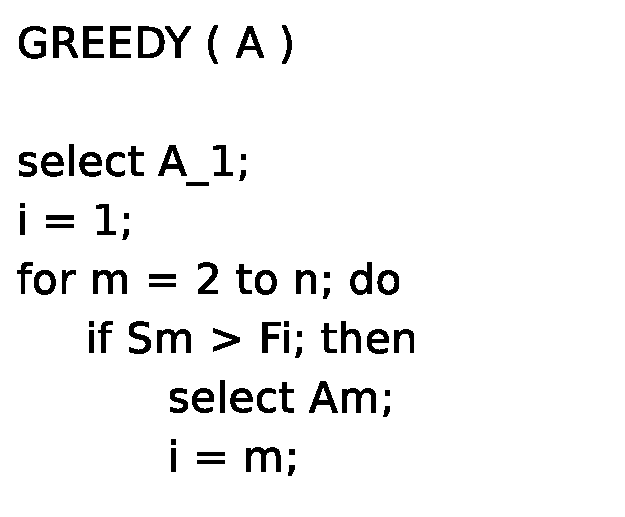
\includegraphics[width=1.0\textwidth]{L7-intervalschedulinggreedyalgo2.eps}%
%      \end{minipage}%
% 
%  \end{figure}

\title{CS612  Algorithm Design and Analysis }
\subtitle{ Lecture 16. Paging problem 
\footnote{The slides are made based on Algorithm Design, Randomized algorithm by R. Motwani and P. Raghavan, and a lecture by T. Chan. } }
\author{Dongbo Bu \\
\ \\
{\small Institute of Computing Technology \\ 
Chinese Academy of Sciences, Beijing, China}}

\date{}

\begin{document}
%\begin{CJK}{UTF8}{cyberbit}

\frame[allowframebreaks]{\titlepage}

\frame{
\frametitle{Outline}
\begin{itemize}
\item Introduction
\item Greedy algorithm: Furthest-Future principle; 
\item Label on-line algorithm framework;
\item The performance of LRU principle;
\item A randomized on-line algorithm (Fiat et al '91);
\end{itemize}
}

\frame[allowframebreaks]{
\frametitle{ {\sc Paging } problem }

\begin{block}{}
{\bf INPUT: } \\
Given a sequence of requests $r_1, r_2, ..., r_n$, and a cache of size $k$; \\
{\bf OUTPUT: } \\ 
schedule the eviction decisions to reduce cache-missing as much as possible. 
\end{block}

}



\frame[allowframebreaks]{
\frametitle{ An example }
An eviction sequence: 
 see a fig.
}

\frame[allowframebreaks]{
\frametitle{ A dynamic-programming method } 
\begin{itemize}
 \item Subproblem: finding the optimal evictions for requests $r_i...r_n$ when cache contents are $c_1,c_2,...,c_k$, $c_i \in \Sigma, |\Sigma| = m $. 
 \item Let $OPT(i, c_1,c_2,..,c_k)$ be the optimal solution value to the subproblem. We have the following recursion: 
  $OPT(i, c_1,c_2,...,c_k) = \min 
\begin{cases}
 OPT(i+1, c_1', c_2',...,c_k'  ) + 1  \\ 
 OPT(i+1, c_1,c_2,...,c_k)  
\end{cases}
$
and $OPT(n, c_1,c_2,...,c_k) = 0$. \\
 Here, $c_1', c_2',...,c_k' $ differs from $c_1, c_2,...,c_k$ at only one page.  
\end{itemize}
Time-complexity: DP table size: $O(n C_m^k )$. Filling each entry takes $k(m-k)+1$ time. 
}

\frame[allowframebreaks]{
\frametitle{ A greedy solution: Furthest-Future principle (L. Belady, '66)}
FF rule: evicts the farthest-future element; 

Furthest-Future eviction sequence $S_{FF}$: 
 see a fig.

\begin{Theorem}
 $S_{FF}$ incurs no more missing than any other schedule $S^*$ and hence is optimal.
\end{Theorem}
Proof: \\
\begin{itemize}
 \item Exchange argument again!. 
 \item Basic idea: From an optimal schedule $S^*$, we generate a series of schedule $S_1,S_2,...,S_n$, such that: \begin{enumerate}
      \item The first $i$ evictions of $S_i$ are the same to that of $S_{FF}$. Thus, $S_n = S_{FF}$. 
      \item $S_{i+1}$ incurs no more missing than $S_i$. 
   \end{enumerate}

 \begin{figure}
        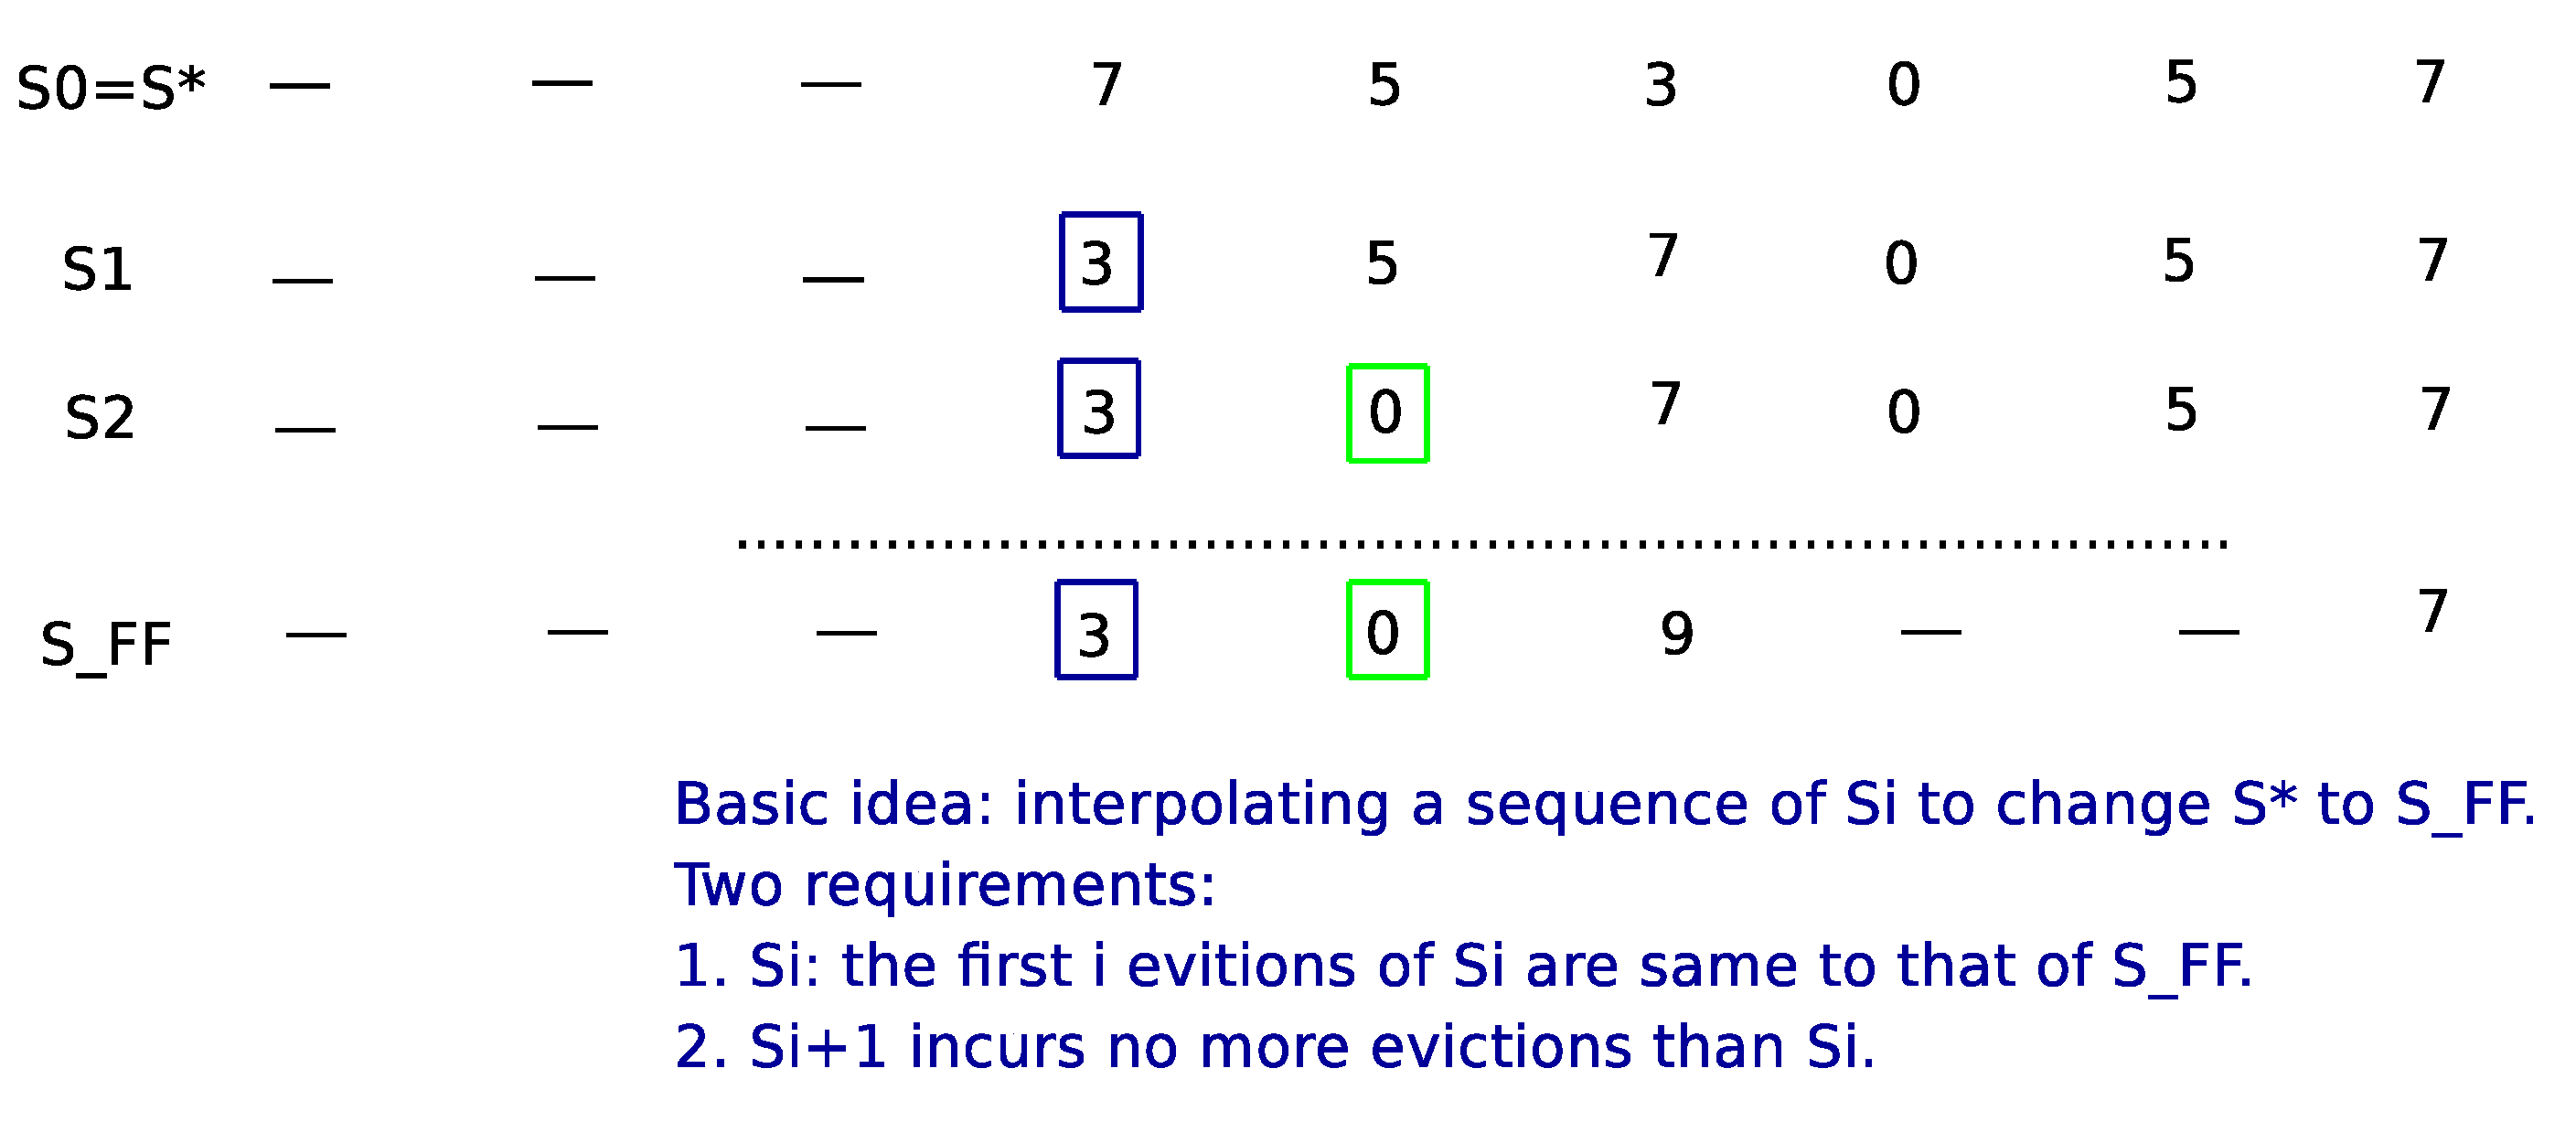
\includegraphics[width=4.2in]{L16-cacheproofidea.eps}
 \end{figure}
\end{itemize}

\begin{itemize}

 \item Difficulty: how to construct $S_{i+1}$ based on $S_i$? 
 \begin{enumerate}
  \item Consider the $j+1$-th request $d$. $S_i$ and $S_{FF}$ have the same cache content till now. 
  \item Suppose $S_i$ evicts $f$ but $S_{FF}$ evicts $e \neq f$. We design $S_{i+1}$ as follows: 
  \item $S_{i+1}$ evicts $e$ at the $j+1$-th step. Now, $S_{i+1}$ and $S_i$ has different cache content.
  \item $S_{i+1}$ simulates the actions of $S_i$ from $j+2$ step until the following two events occurs: 
  \item Case 1: request $g \neq e, f$, and $S_i$ evict $e$. \\ We let $S_{i+1}$ evict $f$. The cache are same now. Thus, we can copy the remaining of $S_i$ to $S_{i+1}$. 
  \item Case 2: request $f$ and $S_i$ evicts $e'$. \\ 
        We let $S_{i+1}$ evict $e'$, too. And fill $e$ if needed. 
 \end{enumerate}
Key: the Furthest-Future principle ensures that before an request of $e$, there should be a request of $f$ (Case 1). 
\end{itemize}

} 

\frame{
Case 1: 
 \begin{figure}
        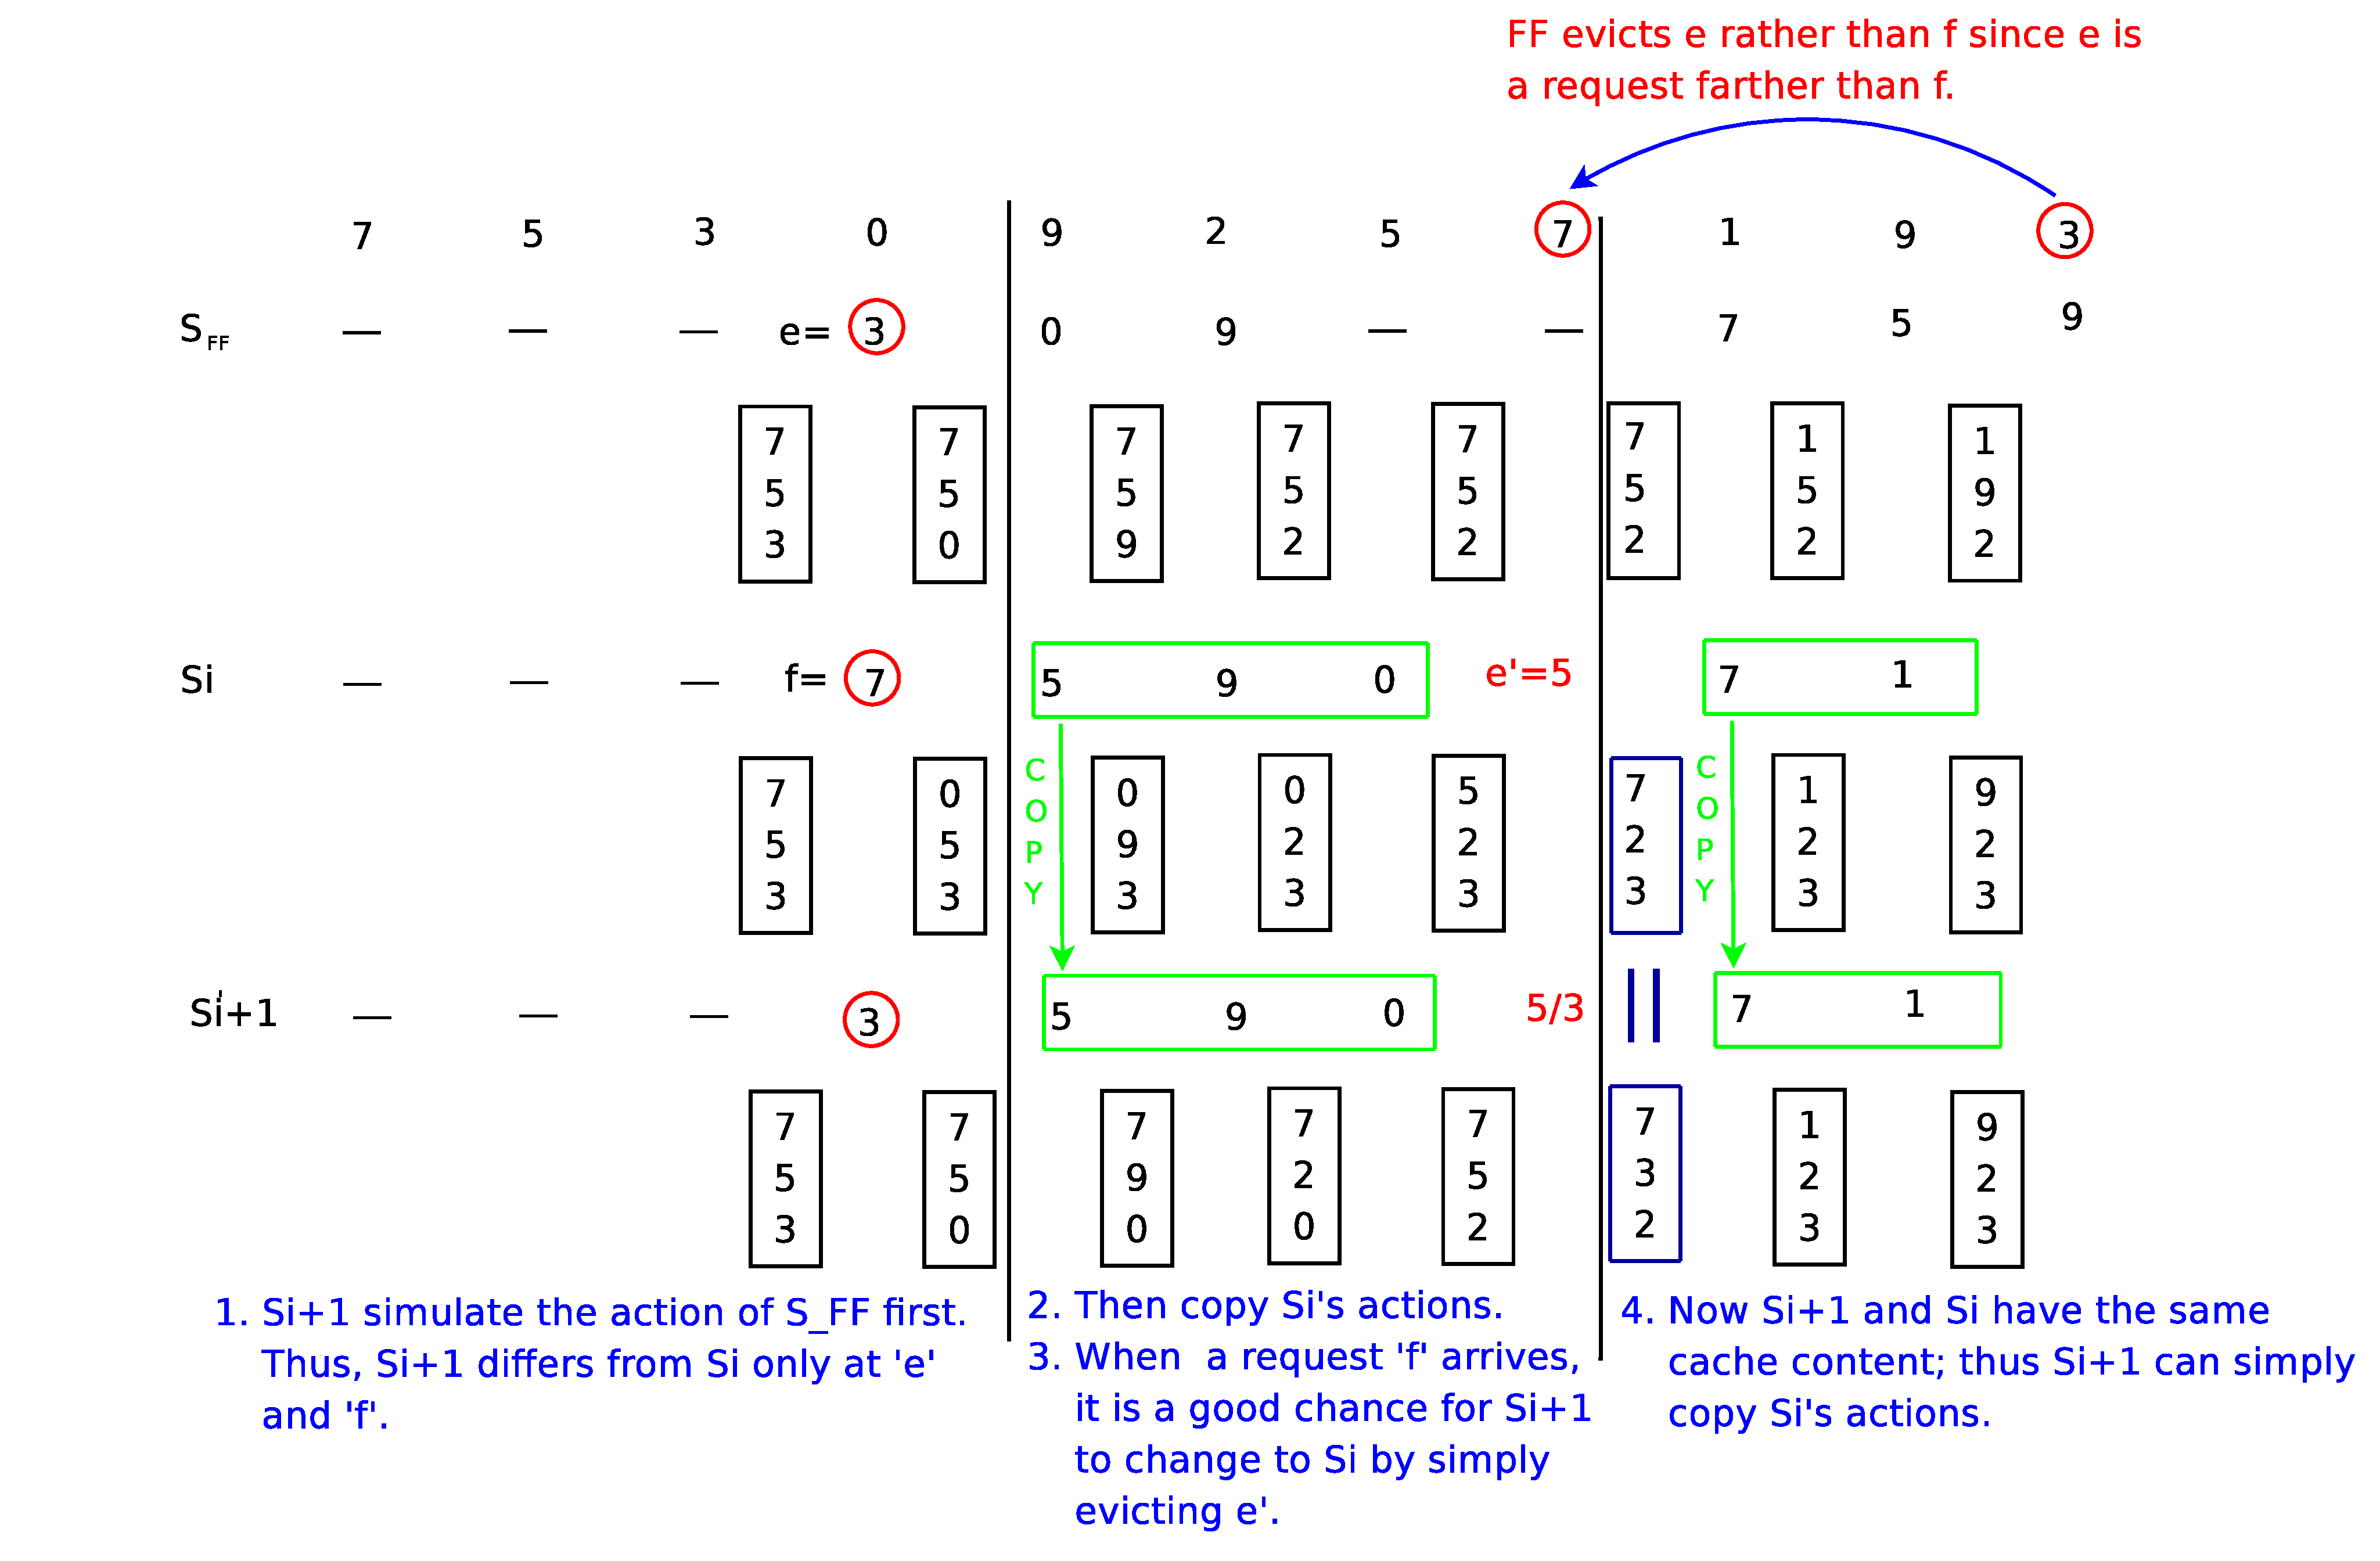
\includegraphics[width=4.3in]{L16-LRUcase1.eps}
 \end{figure}
}
\frame{
Case 2: 
 \begin{figure}
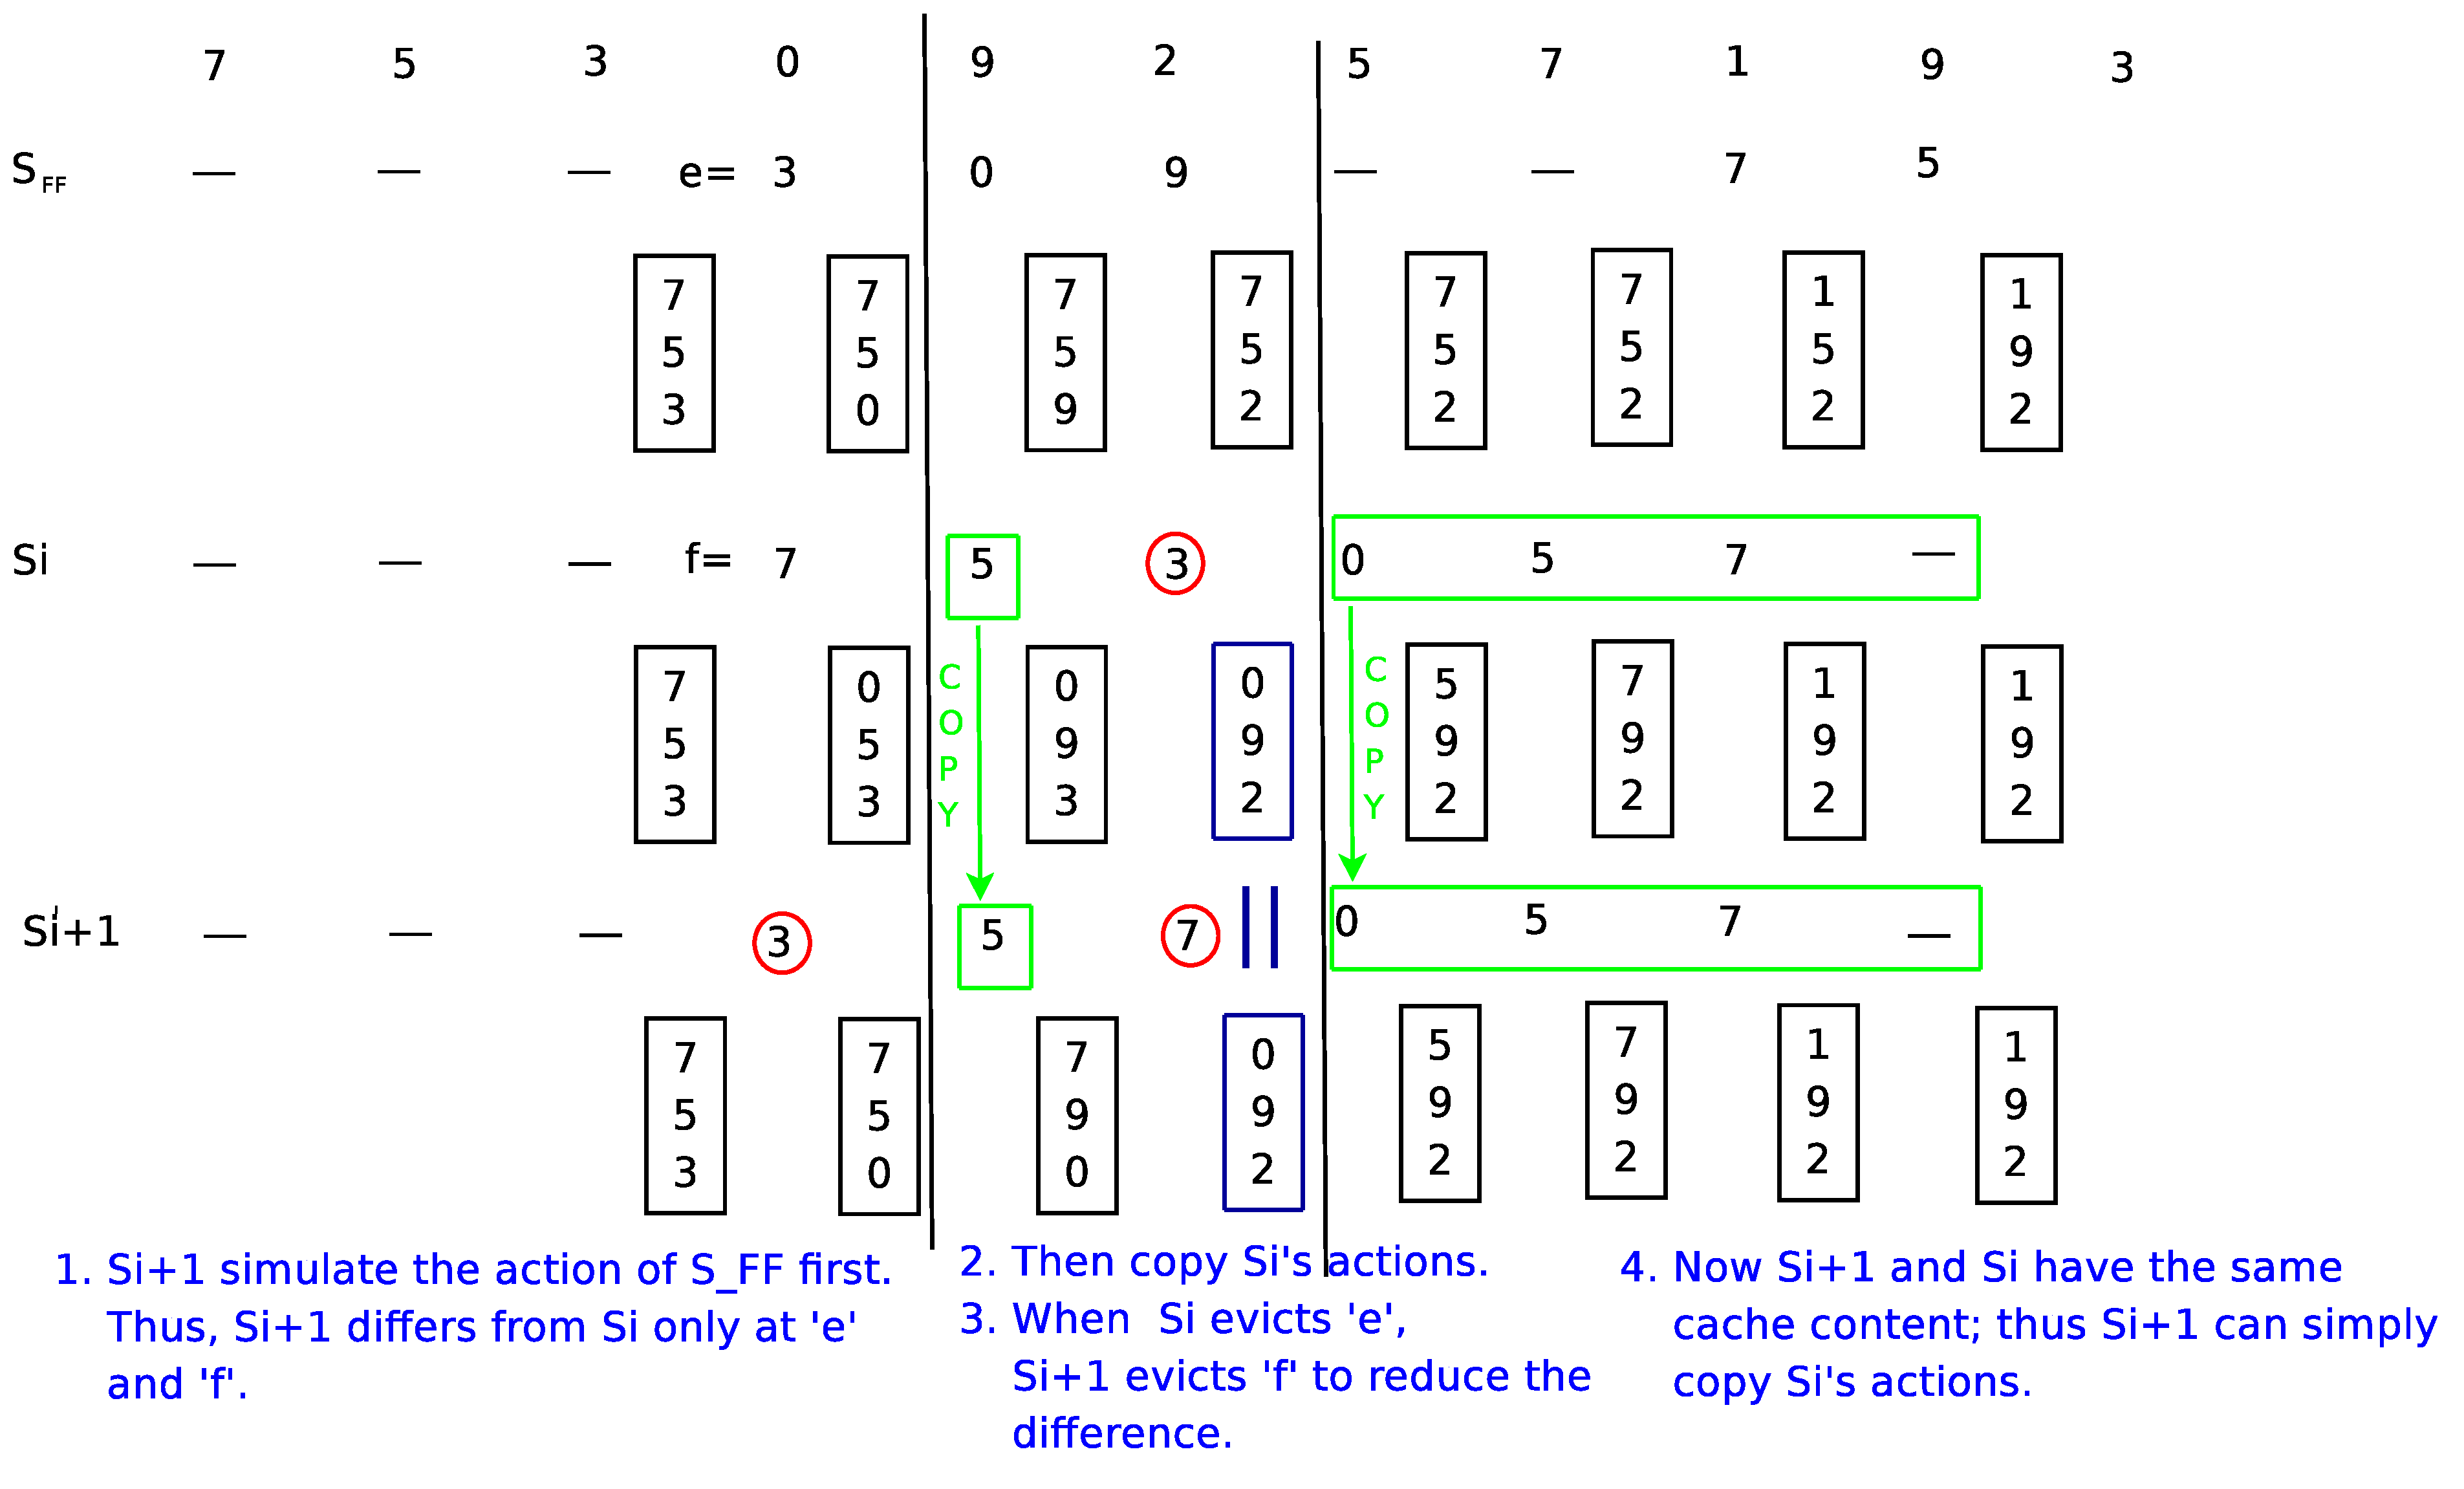
\includegraphics[width=4.3in]{L16-LRUcase2.eps}
 \end{figure}
}

\frame{
\frametitle{From FF to LRU}
\begin{itemize}
 \item 
LRU: least recently used. \\
\item Intuition: ``longest in the past rather than the farthest in the future'' since we have no idea of the future requests. 
\item Reason: locality of reference, i.e., a program will generally keep accessing the things it has just been accessing.
\end{itemize}
}

\frame[allowframebreaks]{
\frametitle{Theoretical analysis of LRU principle (Sleator and Tarjan ) }

Key idea: divide the requests into ``phases''. Each phase consists of a set of evictions.  

A Label-based algorithm framework: 
\begin{enumerate}
 \item initially make all pages in cache as ``old''; 
 \item when a request of page $P$ arrives, 
 \item \quad mark $P$ ``recent''; 
 \item \quad if $P$ is not in cache
 \item \quad \quad if all cache pages are ``recent'',
\item \quad \quad remark all pages ``old'', and begin a new phase; 
\item \quad choose an old page $q$ to evict; 
\end{enumerate}
\textcolor{red}{Old: the pages have already been loaded before this phase. \\
 Recent: the pages are loaded in this phase. } 
\begin{figure}
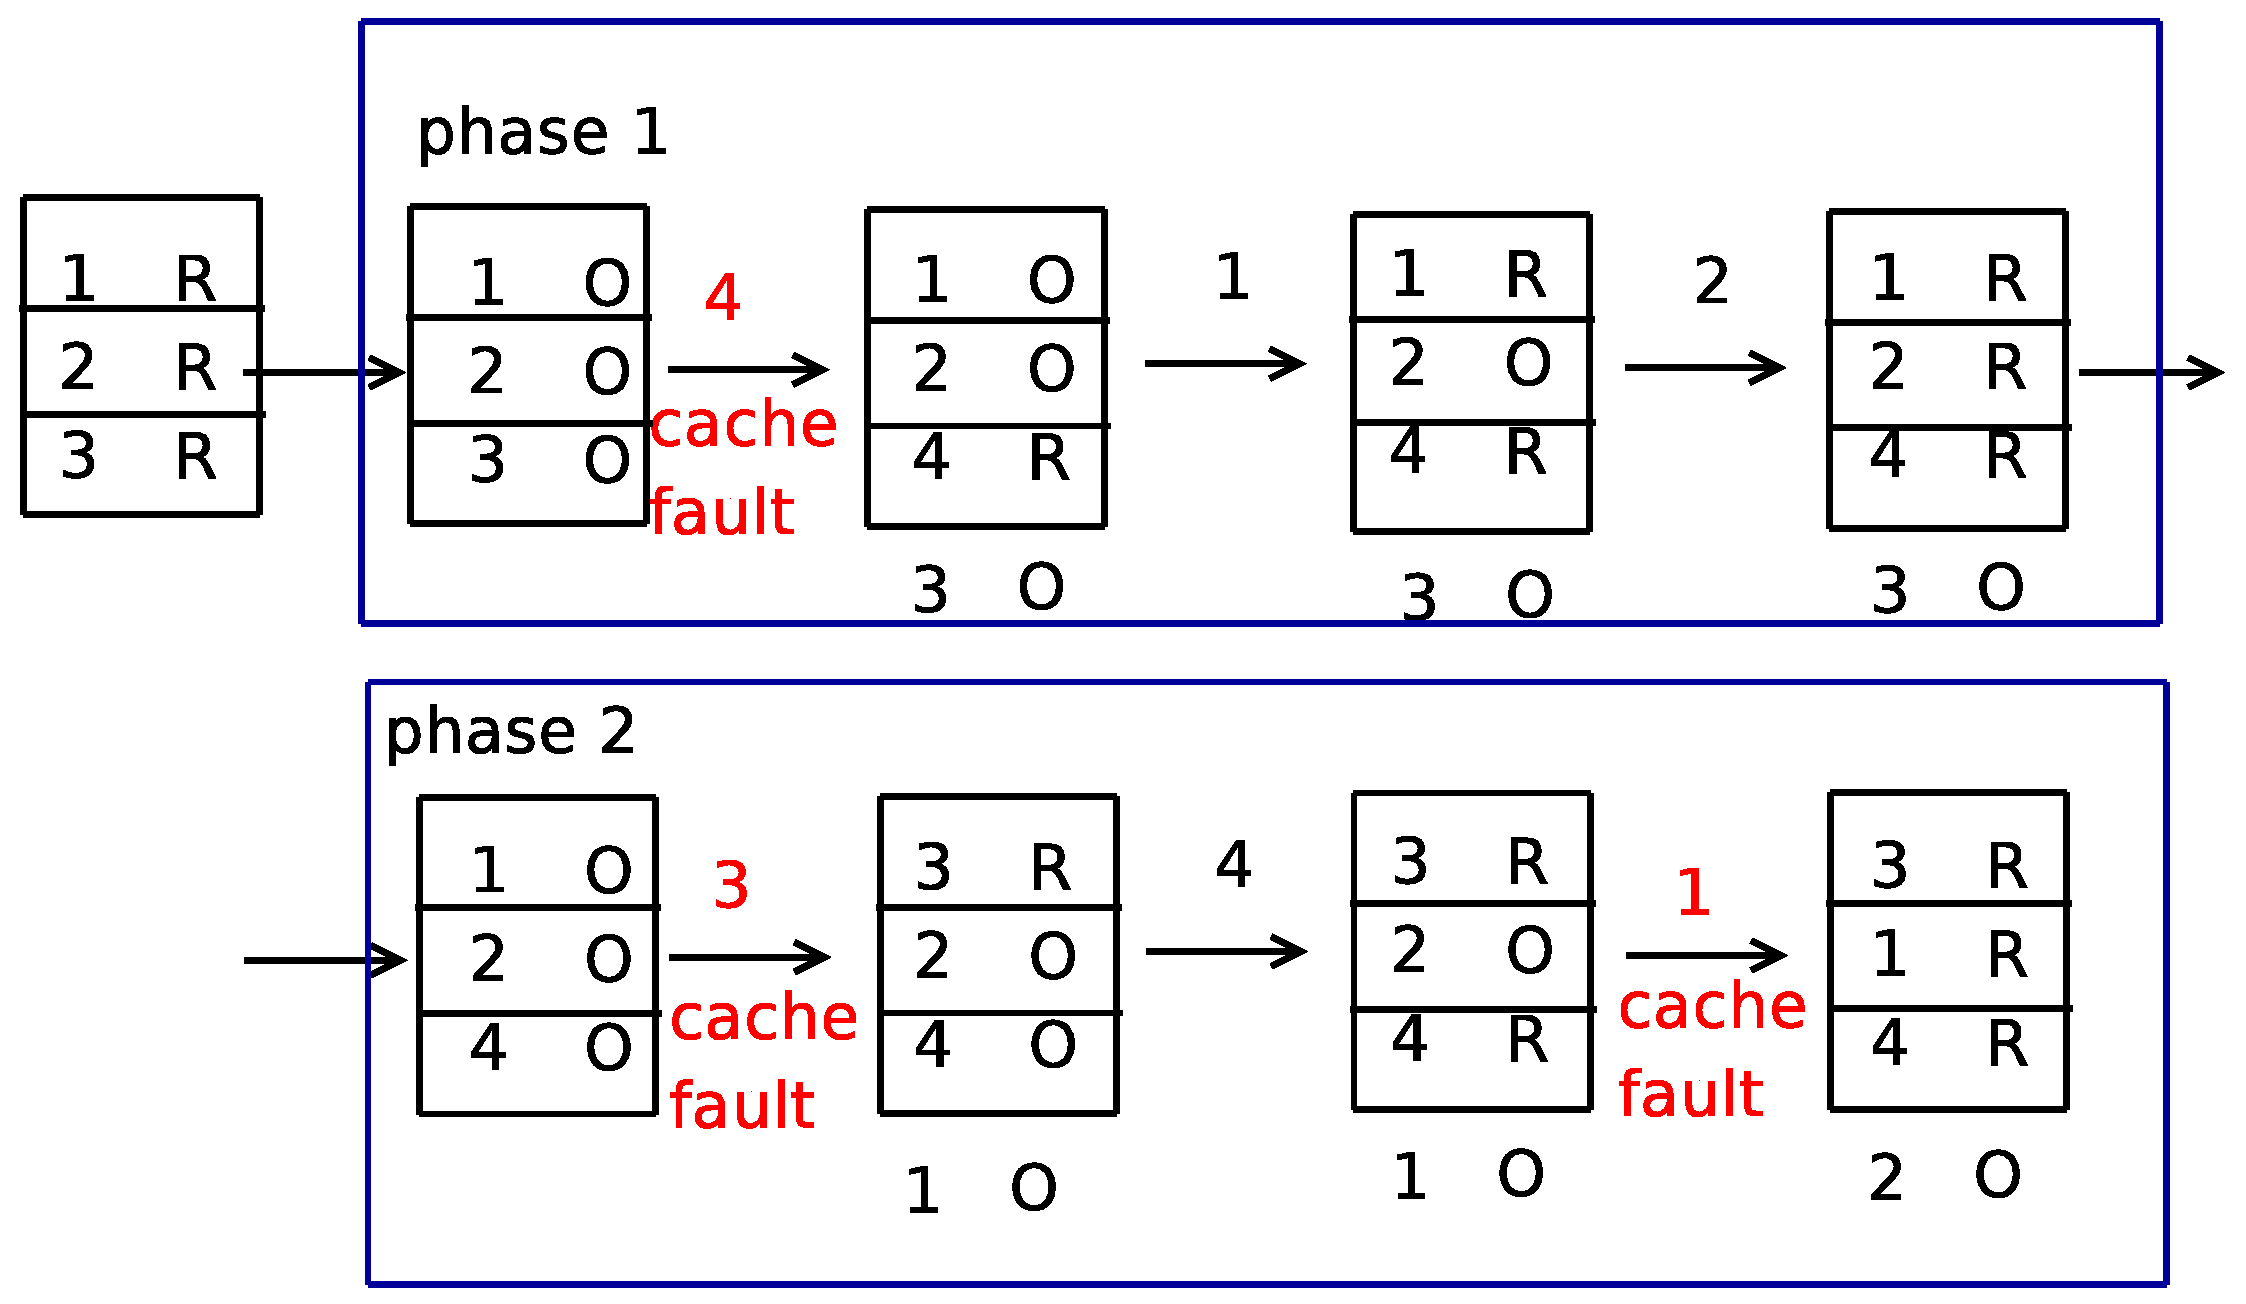
\includegraphics[width=4in]{L16-cachelabelalgoexample.eps}
 \end{figure}

Analysis: \\
Suppose there are $r$ phases. 
\begin{itemize}
 \item Fact 1: Every phase contains $k$ distinct requests. (Reason: when a page changes from ``Old'' to ``Recent'', it will stay in cache till the phase ends.) 
 \item Fact 2: At each phase, there are at most $k$ evictions. Thus, there are at most $rk$ evictions.  (Intuition: evicting a page cause a page remarking from  ``Old'' to ``Recent''.)
 \item Fact 3: An optimal solution incurrs at least $r-1$ missing. (Reason: the first request of a phase $i$ cause a remarking of a page from ``Old'' to ``Recent''. )
 \item Therefore, the ratio of any Label-based algorithm is $k$. 
\end{itemize}

Worst-case: repeating a cycle of requests $1,2,...,k+1$ when cache size is $k$. 

Note: LRU is a Label-based method. 

}

\frame[allowframebreaks]{
\frametitle{ A randomize algo }
Algo: choose a ``random'' old page to evict. 
\begin{Theorem}
Let denote the minimal eviction number as $F^*$. The expected number of evictions of RandomEvition algorithm is at most $2\ln k F^*$. 
\end{Theorem}
Proof: \\
Consider phase $i$. 
 \begin{itemize}
  \item Let $A$ be the cache content at beginning. Sort $A$ according to the request order in this phase, say $A=\{a_1,a_2,...a_k\}$
  \item Let $b_i$ be the requests that are not in $A$. 
  \item When $a_j$ is requested, and $a_j$ is marked ``Old''; (Reason: the case that $a_j$ is ``Recent'' is omited since it causes no cache fault.)
    \item \quad $\#OldPages = k-(j-1)$;  (Reason: $a_1,a_2,...,a_{j-1}$ are marked as ``Recent''.)
  \item \quad $\#OldPagesInCache = k - (j-1) - |b_i| $;  (Reason: a request in $b_i$ evicts an ``Old'' page out of cache.)
 \end{itemize}
Pages in cache are in random. Thus, we have: 
\begin{itemize}
 \item $\Pr( a_j \text{ is in cache } ) \geq \frac{ k-(j-1)- | b_i |}{ k-(j-1)} $;
 \item $\Pr( a_j \text{ is NOT in cache } ) \leq 1 - \frac{ k-(j-1)- | b_i |}{ k-(j-1)} $ (cache missing);
 \item \begin{eqnarray} 
 E( \#missing)  &\leq& b_i + \sum_{j=1}^k \frac{ | b_i |}{k-(j-1)} \\       
&=& | b_i | \log( k - (j-1) ) \\
&=&O(\log(k))
       \end{eqnarray}
\end{itemize}

In phase $i$ and $i+1$, there are $k+b_i$ distinct pages requested. Thus we can bound the number of faults as follows: 
\begin{itemize}
\item $\#missing \geq b_i$ 
\item $\#total-missing \geq \frac{1}{2} \sum_i | b_i | $ 
\item ratio: $\leq 2 \log(k)$. 
\end{itemize}
}

\end{document}
